\documentclass[conference]{IEEEtran}
\IEEEoverridecommandlockouts%

\usepackage[T1]{fontenc}
\usepackage[utf8]{inputenc}
\usepackage{cite}
\usepackage{amsmath,amssymb,amsfonts}
\usepackage{algorithmic}
\usepackage{graphicx}
\usepackage{textcomp}
\usepackage{xcolor}
\usepackage{booktabs,multirow}
\usepackage{tikz}
\usepackage{pgfplots}
\usepackage{hyperref}
\pgfplotsset{compat=1.18}

\def\BibTeX{{\rm B\kern-.05em{\sc i\kern-.025em b}\kern-.08em
		T\kern-.1667em\lower.7ex\hbox{E}\kern-.125emX}}

\title{Supervised Protocol and Parameter Co-Selection for Dynamic IoT Random Access}

\author{
\IEEEauthorblockN{1st Author Name}
\IEEEauthorblockA{\textit{School/Department} \\
\textit{University/Institute}\\
City, Country \\
email@domain.com}
\and
\IEEEauthorblockN{2nd Author Name}
\IEEEauthorblockA{\textit{School/Department} \\
\textit{University/Institute}\\
City, Country \\
email@domain.com}
\and
\IEEEauthorblockN{3rd Author Name}
\IEEEauthorblockA{\textit{School/Department} \\
\textit{University/Institute}\\
City, Country \\
email@domain.com}
}

\begin{document}
\maketitle

\begin{abstract}
Heterogeneous Internet of Things traffic varies in load intensity, burstiness, and periodicity, so fixed random access protocols are often suboptimal in dynamic operation. This paper presents a compact supervised framework for joint protocol and parameter selection under multiple performance objectives. We unify Slotted ALOHA, Slotted ALOHA with Successive Transmission, and Connection Based Access using a common input interface with a protocol identifier and parameter mask. A discrete event simulator generates labels with a two-stage sampling strategy, including coarse global coverage and fine refinement near throughput critical regions. A multi-task neural surrogate then predicts throughput, delay, fairness, and signaling overhead jointly. Online decisions are obtained by fast grid search over the surrogate. Results show accurate prediction and consistent utility gains versus static or single-protocol baselines in non-stationary traffic windows.
\end{abstract}

\begin{IEEEkeywords}
Internet of Things, random access, protocol selection, parameter optimization, multi-task learning, surrogate model.
\end{IEEEkeywords}

\section{Introduction}
Massive Internet of Things (IoT) deployments must support diverse services, from periodic sensing to bursty event reporting. Since contention dynamics are traffic dependent, no single random access protocol remains optimal across all operating points. SA is simple but saturates early~\cite{abramson1970aloha}; SAST improves channel usage through short-term persistence; CBA improves high-load throughput at additional signaling cost.

Most existing methods tune parameters within one protocol family, while practical systems require protocol-level switching as well. This yields a mixed discrete-continuous optimization problem under multiple metrics: throughput, delay, fairness, and signaling overhead. Exhaustive simulation is accurate but expensive.

This paper provides a concise IEEE-style pipeline: unified modeling, simulation dataset generation, multi-task surrogate learning~\cite{caruana1997multitask}, and fast online co-selection.

\section{System Model and Problem Formulation}
We define a unified input vector as
\begin{equation}
\mathbf{X}_{\mathrm{in}}=[\mathbf{x}_{\mathrm{traffic}},\mathbf{x}_{\mathrm{common}},\mathbf{x}_{\mathrm{proto}},\mathbf{m}],
\end{equation}
where $\mathbf{x}_{\mathrm{common}}=[n,T]^\top$ contains network size and time horizon; $\mathbf{x}_{\mathrm{traffic}}$ contains load and temporal statistics; $\mathbf{x}_{\mathrm{proto}}=[a,\mathbf{x}_p^\top]^\top$ contains protocol identity $a\in\mathcal{P}$ and protocol parameters; and $\mathbf{m}$ is a binary validity mask.

For arrival matrix $\mathbf{A}\in\{0,1\}^{n\times T}$, five traffic descriptors are extracted: normalized arrival rate $\hat{\lambda}$, network burstiness $\mathrm{BI}_{\mathrm{net}}$, node burstiness $\mathrm{BI}_{\mathrm{node}}$, network periodicity $\Psi_{\mathrm{net}}$, and node periodicity $\Psi_{\mathrm{node}}$.

Given $\mathbf{X}_{\mathrm{in}}$, the simulator output is
\begin{equation}
\mathbf{y}=S(\mathbf{X}_{\mathrm{in}})=[\lambda_{\mathrm{out}},D,J_T,S],
\end{equation}
where $\lambda_{\mathrm{out}}$, $D$, $J_T$, and $S$ are throughput, delay, Jain fairness~\cite{jain1984quantitative}, and signaling overhead.

After min-max normalization and utility/cost alignment, the scalar utility is
\begin{equation}
U(\tilde{\mathbf{y}})=w_\lambda\tilde{\lambda}_{\mathrm{out}}+w_D\tilde{D}+w_J\tilde{J}_T+w_S\tilde{S},\ \sum_i w_i=1.
\end{equation}
The co-selection objective is
\begin{equation}
\mathbf{x}_{\mathrm{proto}}^*=\arg\max_{\mathbf{x}_{\mathrm{proto}}\in\mathcal{X}} U\!\left(\mathrm{norm}\left(S(\mathbf{X}_{\mathrm{in}})\right)\right),\ \text{s.t. } S\le S_{\max}.
\end{equation}

\section{Unified Framework}
\subsection{Protocol Abstraction and Execution}
The protocol set is $\mathcal{P}=\{\mathrm{SA},\mathrm{SAST},\mathrm{CBA}\}$. SA and SAST use access probability $q$; CBA uses $(q,M)$ with $M\in\{1,2,4\}$. A unified simulator executes slot-wise arrival generation, access decisions, channel resolution, queue updates, and metric accounting.

\begin{figure}[t]
\centering
\begin{tikzpicture}[font=\footnotesize, node distance=1.0cm and 0.9cm, >=latex]
	\tikzstyle{blk}=[draw, rounded corners, align=center, minimum height=0.9cm, minimum width=2.55cm]
	\node[blk] (traffic) {Traffic Features\\$\hat{\lambda},\mathrm{BI},\Psi$};
	\node[blk, right=of traffic] (proto) {Protocol Pool\\SA / SAST / CBA};
	\node[blk, right=of proto] (sim) {Unified Simulator\\$S(\mathbf{X}_{\mathrm{in}})$};
	\node[blk, below=of sim] (dataset) {Labeled Dataset};
	\node[blk, left=of dataset] (mtl) {MT-DNN Surrogate\\$f_\phi$};
	\node[blk, left=of mtl] (search) {Online Search\\$\arg\max U$};
	\draw[->] (traffic) -- (proto);
	\draw[->] (proto) -- (sim);
	\draw[->] (sim) -- node[right] {$\mathbf{y}$} (dataset);
	\draw[->] (dataset) -- (mtl);
	\draw[->] (mtl) -- (search);
	\draw[->, dashed] (search.north) |- (proto.south);
\end{tikzpicture}
\caption{Unified protocol-parameter co-selection pipeline.}
\label{fig:framework}
\end{figure}

\subsection{Surrogate Learning and Online Search}
We train a hard-parameter-sharing multi-task model: shared hidden layers with normalization, GELU, and dropout, followed by four task heads. At runtime, the learned surrogate $f_\phi$ replaces expensive simulation,
\begin{equation}
\mathbf{x}_{\mathrm{proto}}^*=\arg\max_{\mathbf{x}_{\mathrm{proto}}\in\mathcal{X}}U\big(f_\phi(\mathbf{X}_{\mathrm{in}})\big),
\end{equation}
and candidate configurations are evaluated by fast grid search.

\section{Simulations}
\subsection{Dataset Generation}
A two-stage sampling strategy is used: (1) coarse sampling over feasible load ranges per protocol; (2) fine sampling around transition and peak regions identified in stage 1. Traffic types include uniform, bursty, and periodic arrivals. Each configuration is repeated with independent seeds and averaged labels.

\begin{table}[t]
\centering
\caption{Dataset summary for surrogate training.}
\label{tab:dataset}
\begin{tabular}{lccc}
\toprule
Protocol & Configurations & Valid Samples & $\hat{\lambda}$ Range \\
\midrule
SA   & 400 & 395 & [0.01, 0.50] \\
SAST & 800 & 782 & [0.01, 0.70] \\
CBA  & 800 & 791 & [0.01, 0.70] \\
\midrule
Total & 2000 & 1968 & N/A \\
\bottomrule
\end{tabular}
\end{table}

\subsection{Evaluation Settings}
Three strategies are compared under dynamic windows: 
\textit{(i)} fixed SA ($q=0.01$), 
\textit{(ii)} fixed CBA with parameter tuning only, and 
\textit{(iii)} the proposed dynamic co-selection. 
Default utility weights are $[w_\lambda,w_D,w_J,w_S]=[0.4,0.3,0.2,0.1]$.

\section{Results and Discussion}
\subsection{Surrogate Accuracy}
Table~\ref{tab:error} reports held-out prediction quality. The model is sufficiently accurate for online optimization.

\begin{table}[t]
\centering
\caption{Test performance of multi-task surrogate.}
\label{tab:error}
\begin{tabular}{lccc}
\toprule
Metric & MSE & MAE & $R^2$ \\
\midrule
Throughput $\lambda_{\mathrm{out}}$ & 0.0010 & 0.0160 & 0.980 \\
Delay $D$ & 0.0045 & 0.0170 & 0.919 \\
Fairness $J_T$ & 0.0017 & 0.0290 & 0.988 \\
Signaling $S$ & 0.0002 & 0.0121 & 0.994 \\
\bottomrule
\end{tabular}
\end{table}

\subsection{Dynamic Utility Gains}
Figure~\ref{fig:utility} shows utility over 10 non-stationary windows. The proposed method stays closest to the oracle upper bound and outperforms both baselines.

\begin{figure}[t]
\centering
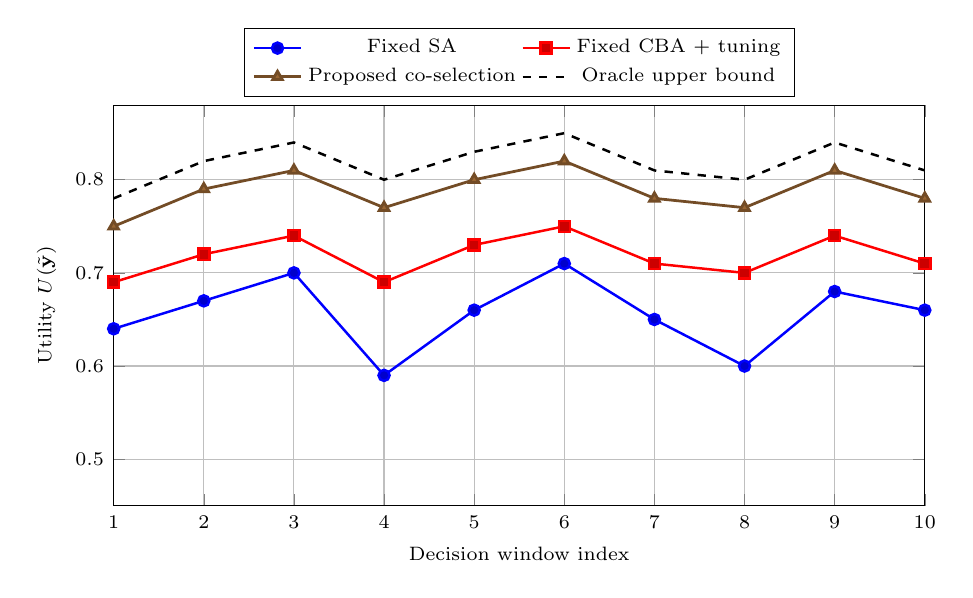
\begin{tikzpicture}
\begin{axis}[
	width=0.98\columnwidth,
	height=0.55\columnwidth,
	xmin=1, xmax=10,
	ymin=0.45, ymax=0.88,
	xlabel={Decision window index},
	ylabel={Utility $U(\tilde{\mathbf{y}})$},
	legend style={font=\scriptsize, at={(0.5,1.02)}, anchor=south, legend columns=2},
	grid=both,
	tick label style={font=\scriptsize},
	label style={font=\scriptsize}
]
\addplot+[mark=*, line width=0.9pt] coordinates {(1,0.64)(2,0.67)(3,0.70)(4,0.59)(5,0.66)(6,0.71)(7,0.65)(8,0.60)(9,0.68)(10,0.66)};
\addlegendentry{Fixed SA}
\addplot+[mark=square*, line width=0.9pt] coordinates {(1,0.69)(2,0.72)(3,0.74)(4,0.69)(5,0.73)(6,0.75)(7,0.71)(8,0.70)(9,0.74)(10,0.71)};
\addlegendentry{Fixed CBA + tuning}
\addplot+[mark=triangle*, line width=1.0pt] coordinates {(1,0.75)(2,0.79)(3,0.81)(4,0.77)(5,0.80)(6,0.82)(7,0.78)(8,0.77)(9,0.81)(10,0.78)};
\addlegendentry{Proposed co-selection}
\addplot+[mark=none, dashed, line width=0.9pt] coordinates {(1,0.78)(2,0.82)(3,0.84)(4,0.80)(5,0.83)(6,0.85)(7,0.81)(8,0.80)(9,0.84)(10,0.81)};
\addlegendentry{Oracle upper bound}
\end{axis}
\end{tikzpicture}
\caption{Utility under dynamic traffic windows (higher is better).}
\label{fig:utility}
\end{figure}

\subsection{Protocol Trade-off}
Figure~\ref{fig:tradeoff} highlights typical trade-offs: CBA gives higher throughput with higher signaling cost; SA has lower overhead but lower throughput ceiling; SAST provides a middle regime.

\begin{figure}[t]
\centering
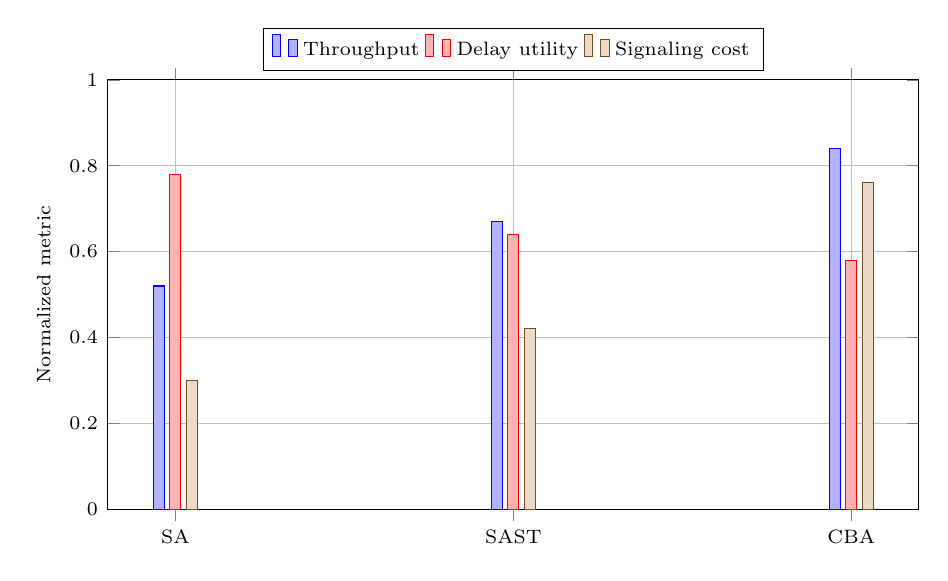
\begin{tikzpicture}
\begin{axis}[
	ybar,
	bar width=4pt,
	width=0.98\columnwidth,
	height=0.58\columnwidth,
	ymin=0, ymax=1.0,
	ylabel={Normalized metric},
	symbolic x coords={SA,SAST,CBA},
	xtick=data,
	legend style={font=\scriptsize, at={(0.5,1.02)}, anchor=south, legend columns=3},
	grid=both,
	tick label style={font=\scriptsize},
	label style={font=\scriptsize}
]
\addplot coordinates {(SA,0.52) (SAST,0.67) (CBA,0.84)};
\addplot coordinates {(SA,0.78) (SAST,0.64) (CBA,0.58)};
\addplot coordinates {(SA,0.30) (SAST,0.42) (CBA,0.76)};
\legend{Throughput,Delay utility,Signaling cost}
\end{axis}
\end{tikzpicture}
\caption{Illustrative metric trade-offs across protocols at moderate load.}
\label{fig:tradeoff}
\end{figure}

\section{Conclusion}
This paper presented a supervised method for protocol-parameter co-selection in dynamic IoT random access. A unified interface and two-stage sampling produced a compact but informative dataset, and a multi-task surrogate enabled millisecond-level decision making. Simulations demonstrated robust prediction quality and clear utility gains over static baselines. Future work includes uncertainty-aware selection and hardware-in-the-loop validation.

\bibliographystyle{IEEEtran}
\bibliography{refs}

\end{document}
